% !TeX root = main.tex

\hypertarget{curve-sketching}{%
\section{Curve Sketching}\label{curve-sketching}}

\hypertarget{limits-at-infinity}{%
\subsection{Limits at Infinity}\label{limits-at-infinity}}

\begin{definition}

Let \(f\) be a function defined on an interval \((a, \infty)\). If the
values of \(f(x)\) becomes arbitrarily close to \(L\) as \(x\) becomes
sufficiently large, we say the function \(f\) has a \textbf{limit at
infinity} and write \(\lim\limits_{x\to \infty}f(x)=L.\)

Let \(f\) be a function defined on an interval \((-\infty, a)\). If the
value of \(f(x)\) becomes arbitrarily close to \(L\) for as \(-x\)
becomes sufficiently large, we say that the function \(f\) has a
\textbf{limit at negative infinity} and write
\(\lim\limits_{x\to -\infty}f(x)=L.\)

\end{definition}


\begin{remark}

For limits at infinity, limit laws still work.

\end{remark}

\begin{example}

Consider the function \(f(x)=2+\frac1x\). Find
\(\lim\limits_{x\to -\infty}f(x)\) and
\(\lim\limits_{x\to \infty}f(x)\).

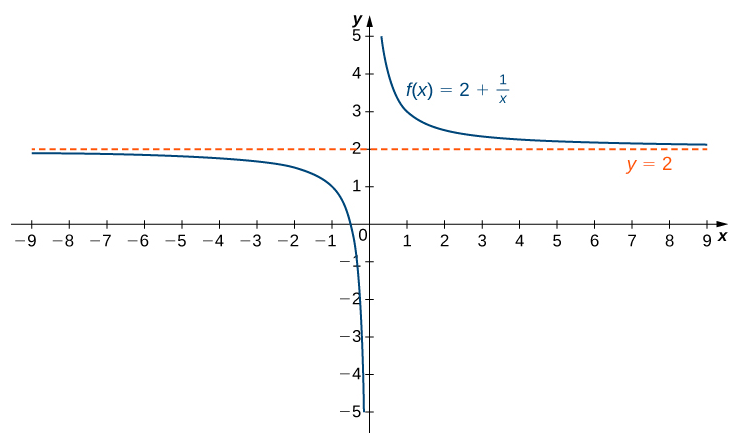
\includegraphics[width=0.9\textwidth]{img/image-20200415101551680.png}

\end{example}
\vspace*{2\baselineskip}

\begin{theorem}

Let \(p(x)=a_nx^n+a_{n-1}x^{n-1}+\cdots + a_{1}x+a_0\) and
\(q(x)=b_m x^m+b_{m-1}x^{m-1}+\cdots + b_1x+b_0\) are two polynomials.
Then \[
\lim\limits_{x\to \pm\infty}\frac{p(x)}{q(x)}=
\begin{cases}
0 & \text{if}~ n<m\\
\frac{a_n}{b_m} & \text{if}~ n=m\\
\end{cases}
\] When \(n>m\), the limit at infinity is an infinite limit.

\end{theorem}

\textbf{Recall:} A function \(f\) has an infinite limit at \(a\) if
\(\lim\limits_{x\to a}f(x)=\infty ~\text{or}~-\infty\), where \(a\) can
be a finite number, infinity or negative infinity.

\begin{example}

Find the limits
\(\lim\limits_{x\to \infty} \frac{x^4 - 4x^3+1}{2 - 2x^2 - 7x^4}\).

\end{example}
\vspace*{6\baselineskip}

\begin{example}

Find the limit
\(\lim\limits_{x\to -\infty} =\frac{x^2+\cos(x^3)}{2 - 2x^3}\).

\end{example}
\vspace*{6\baselineskip}

\hypertarget{asymptotes}{%
\subsection{Asymptotes}\label{asymptotes}}

\begin{definition}

Let \(f\) be a function defined for \(x\) or \(-x\) sufficiently large.
If \(\lim\limits_{x\to \infty}f(x)=L\) or
\(\lim\limits_{x\to -\infty}f(x)=L\), we say the line \(y=L\) is a
\emph{horizontal asymptote} of \(f\).

Let \(f\) be a function defined near \(x=a\). If
\(\lim\limits_{x\to a^-}f(x)=\infty~\text{or}~-\infty\) or
\(\lim\limits_{x\to a^+}f(x)=\infty ~\text{or}~-\infty\), we say the
line \(x=a\) is a \emph{vertical asymptote} of \(f\).

\end{definition}

\begin{example}

Consider the function \(f(x)=1-\frac1{x-1}\). Find all horizontal and
vertical asymptotes.

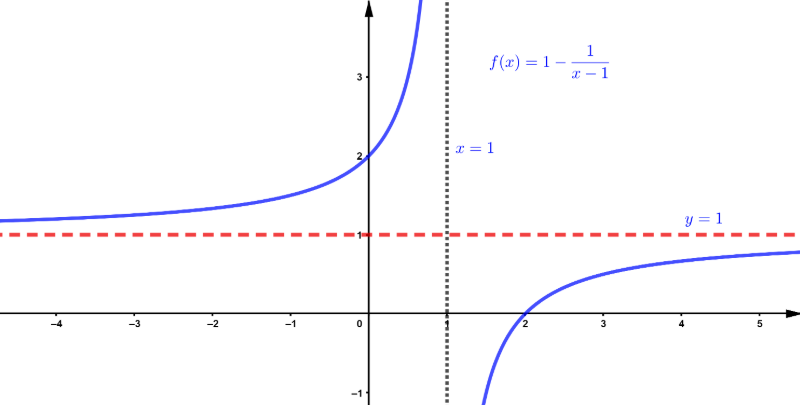
\includegraphics[width=0.9\textwidth]{img/image-20200415104515572.png}

\end{example}
\vspace*{6\baselineskip}

\begin{example}

Determine the horizontal asymptote(s) and the vertical asymptote(s) for
the function \(f\) if they exist.

\begin{enumerate}
\item
  \(f(x)=3-\frac{5}{x^2}\)
\item
  \(f(x)=\frac{\sin x}{x}\)
\end{enumerate}

\end{example}

\hypertarget{slant-asymptote}{%
\subsection{Slant Asymptote}\label{slant-asymptote}}

\begin{definition}

A line \(y=mx+b\) is a \textbf{slant asymptote} of a function \(f\) if

\[\lim\limits_{x\to \infty}[f(x)-(mx+b)]=0  ~ \text{or} ~ \lim\limits_{x\to \infty}[f(x)-(mx+b)]=0.\]

\end{definition}

\begin{example}

Determine if the function \(f(x)=\frac{x^2+x-1}{2x+4}\) has a slant
asymptote. If so, find it.

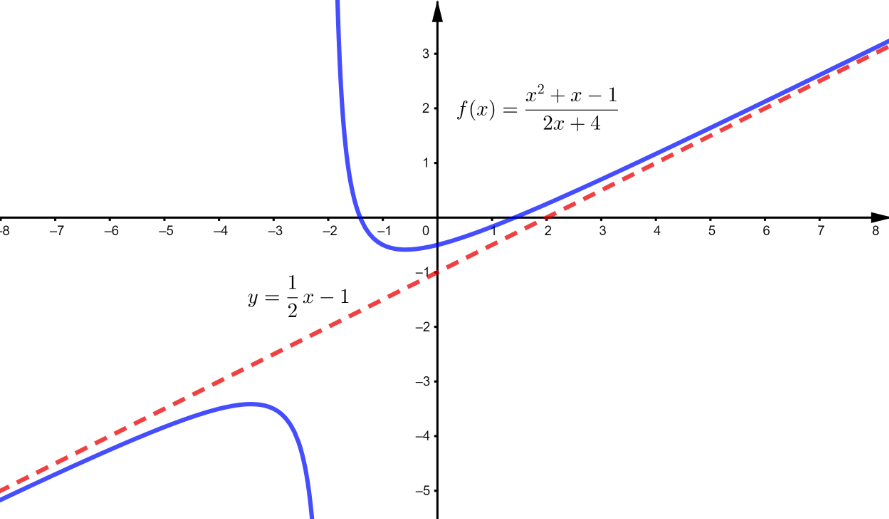
\includegraphics[width=0.9\textwidth]{img/image-20200415114002896.png}

\end{example}
\vspace*{6\baselineskip}

\hypertarget{a-guideline-to-curve-sketching}{%
\subsection{A guideline to curve
sketching}\label{a-guideline-to-curve-sketching}}

\begin{enumerate}
\item
  Find the domain of \(f\).
\item
  Solve for \(x\) from \(f(x)=0\) to find the \(x\)-intercepts and find
  the \(y\)-intercept \((0, f(0))\).
\item
  Determine if the function has any symmetry:

  \begin{enumerate}
  \def\labelenumii{(\alph{enumii})}
  \item
    Is \(f\) an even function, i.e.~\(f(-x)=f(x)\) for all \(x\)?
  \item
    Is \(f\) an odd function, i.e.~\(f(-x)=-f(x)\) for all \(x\)?
  \item
    Is \(f\) a periodic function, i.e.~there is a constant \(p\) such
    that \(f(x+p)=f(x)\) for all \(x\)?
  \end{enumerate}
\item
  Evaluate \(\lim\limits_{x\to -\infty} f(x)\) and
  \(\lim\limits_{x\to \infty} f(x)\) to determine the end behavior of
  \(f\). Find horizontal asymptotes if they exist.
\item
  Find vertical asymptotes if they exist.
\item
  Find slant asymptotes, i.e.~\(y=mx+b\) such that
  \(\lim\limits_{x\to \pm\infty}(f(x)-(mx+b))=0\). Note that
  \(m=\lim\limits_{x\to \infty}\frac{f(x)}{x}\) and
  \(b=\lim\limits_{x\to \infty}(f(x)-mx)\).
\item
  Calculate \(f'\) and find all critical values if they exist. Determine
  the intervals of increasing and decreasing.
\item
  Determine local extrema if they exist.
\item
  Calculate \(f''\). Determine the intervals of concave up and concave
  down. Determine inflection points if they exist.
\item
  Sketch the curve using the above information.
\end{enumerate}

\begin{example}
  
Sketch a graph of \(f(x)=(x - 1)^2(x+1).\)

\end{example}
\vspace*{6\baselineskip}


\begin{example}
  
Sketch the graph of \(f(x)=\frac{x+2}{x^2+5x+4}\).

\end{example}
\vspace*{6\baselineskip}

\subsection{Practice}

\begin{exercise}

Find the limits \(\lim\limits_{x\to -\infty}\frac{x}{x - 2}\).

\end{exercise}
\vspace*{6\baselineskip}

\begin{exercise}

Find the limit \(\lim\limits_{x\to -\infty}\frac{\sqrt{4x^2 - 1}}{x+2}\).

\end{exercise}
\vspace*{6\baselineskip}

\begin{exercise}

Find the limit
\(\lim\limits_{x\to \infty}\frac{\sqrt{x^5+1}}{x^2 - \sqrt{x}+1}\).

\end{exercise}
\vspace*{6\baselineskip}

\begin{exercise}

Determine the horizontal asymptote(s) and the vertical asymptote(s) for
the function \(f\) if they exist.

\begin{enumerate}
\item
  \(f(x)=\frac{x}{1 - x^2}\)
\item
  \(f(x)=\frac{x\sin x}{x^2 - 1}\)
\end{enumerate}

\end{exercise}

\begin{exercise}

Determine if the function \(f(x)=\frac{x^2+7x+6}{x+2}\) has a slant
asymptote. If so, find it.

\end{exercise}
\vspace*{6\baselineskip}

\begin{exercise}

Sketch the graph of \(f(x)=x^3 - 3x^2+4\).

\end{exercise}
\vspace*{6\baselineskip}

\begin{exercise}

Sketch the graph of \(f(x)=\frac{2x+3}{x^{2}+8x+12}\).

\end{exercise}
\vspace*{6\baselineskip}

\begin{exercise}

Sketch the graph of \(f(x)=\sqrt{x^2 - 5x+4}\).

\end{exercise}

